\section{Exact Stochastic Simulation Algorithms}

\subsection{Exponential waiting times and competing stochastic events}
So far we have made a strong emphasis on the correspondence between the deterministic and the stochastic description of the temporal dynamics of a system. The Gillespie algorithm is a robust method to generate stochastic replicates of the temporal dynamics of a system. Suppose we deal with a single population described by the stochastic variable $N$, number of individuals. The method is exact in the sense that it generates realizations of the continuous-time Markov process defined by the prescribed elementary events and their transition rates. For the linear processes discussed so far, averaging over many independent stochastic realizations recovers the deterministic equation for the mean population size. In nonlinear systems, however, the equation for the mean may involve higher moments, so the usual deterministic approximation need not coincide with the exact stochastic mean. Individual stochastic trajectories fluctuate around, and sometimes depart substantially from, deterministic predictions.  
\smallskip

As described in section \ref{subsection:Poisson_Process}, let us assume we have a Poissonian counting process. The line in front the counter keeps increasing due to the constant arrival of individuals at rate $\lambda$. Can we generate stochastic replicates of this process? Of course, we can. We will do it by introducing the Gillespie algorithm. Assuming that there were no individuals at the initial time $t=0$, we know that the number of individuals at a certain time $t$ follows a Poissonian distribution:
\begin{equation}
\Pb(n, t) =  \frac{(\lambda t)^n}{n!} e^{-\lambda t}
\label{Poisson_Distribution}
\end{equation}

Interestingly, there is some non-null probability of having still no individuals after a given time $t$:
\begin{equation}
\Pb(0, t) =  e^{-\lambda t}
\label{Eq_Exp_1}
\end{equation}
which is obtained by making $n=0$ in Eq (\ref{Poisson_Distribution}). The time between two consecutive arrival events can be considered a stochastic variable $T$, which we call the inter-event time.  Since at time $t$ we still have 0 individuals, $\Pb(0, t)$ can be read as the probability that the next arrival occurs at a time larger than $t$. We can then write:
\begin{equation}
\Pb\{T>t\} =  e^{-\lambda t}
\end{equation}
It is also crystal clear that:
\begin{equation}
\Pb\{T<t\} =  1 - e^{-\lambda t}
\end{equation}
Now compare please the last equation with Eq (\ref{Exponential_Distribution}). This comparison is conclusive: $T \sim Exponential(\lambda)$, this is, in words, we can conclude that the stochastic variable $T$, defined as the inter-event time (a.k.a the time-to-the-next-event) follows an exponential distribution of parameter $\lambda$. 
\smallskip

If we know that a random variable follows certain distribution, we can always sample it, i.e., we can use this distribution to draw an individual realization of that variable. When the stochastic variable is continuous, as it is the case for the inter-event time, we can always take a single realization of this stochastic variable by using the so-called inversion method (see Fig \ref{Inversion_Method}). This method uses the cumulative probability distribution (Eq (\ref{Exponential_Distribution})). It draws first a full, uniformly-distributed random number, $\xi$, between 0 and 1, and then, it looks at the time on the horizontal axis that corresponds to this random $\xi$ on the vertical axis\footnote{Here, a full random number, $\xi$, between 0 and 1 means the realization of a stochastic variable, $X$, that follows the uniform distribution between 0 and 1. The cumulative probability distribution of a uniformly distributed random variable, $X$, is then the identity function between 0 and 1, $F(x) = \Pb\{X\,<\,x\}= x$.}  (see Fig \ref{Inversion_Method}). Luckily this can be calculated:
\begin{align*}
 \xi            &= 1 - e^{-\lambda t}            \\
 e^{-\lambda t} &= 1 - \xi                       \\
 -\lambda t     &= \log(1 - \xi)                 \\
          t     &= -\frac{\log(1 - \xi)}{\lambda}
\end{align*}
If $\xi$ is uniformly distributed between 0 and 1, the complementary variable $1-\xi$ will be also uniformly distributed between 0 and 1. We safely define $\Phi \equiv 1-\xi$:
\begin{equation}
 t     = -\frac{\log(\Phi)}{\lambda}
 \label{Random_Time}
\end{equation}

\begin{figure}[t!]
	\centering
	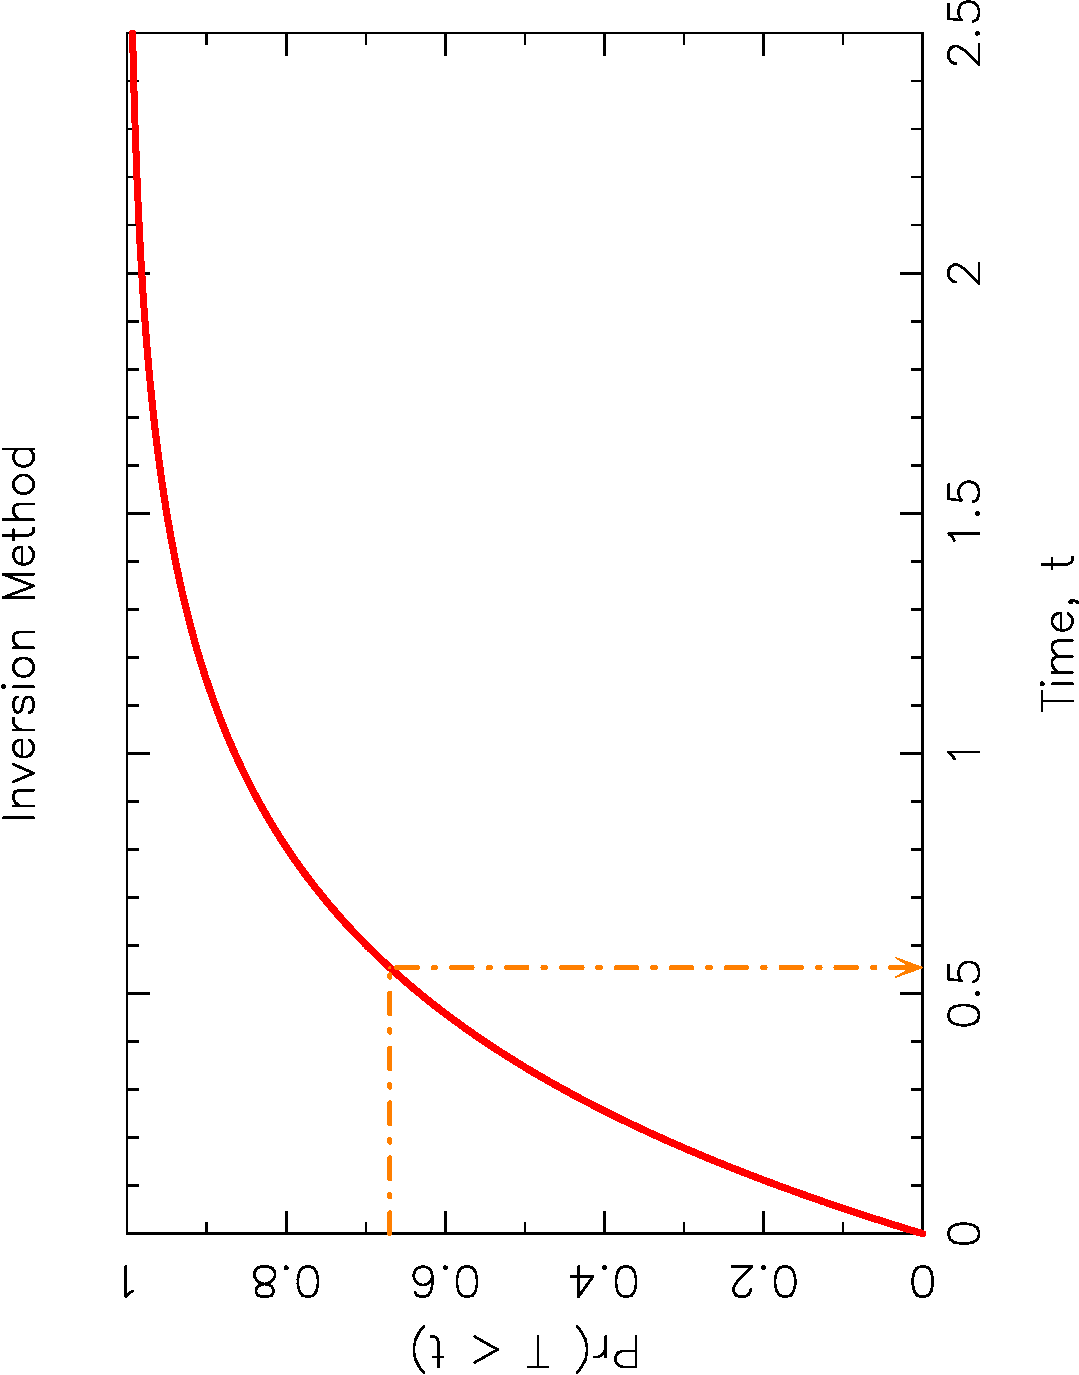
\includegraphics[width=0.6\textwidth,angle=270]{Inversion_Method}
	\caption[Inversion Method]{In order to sample a random variable following a given probability distribution, the inversion method is often used. One generates a uniformly distributed random number between 0 and 1, on the vertical axis, and looks for the corresponding value on the horizontal axis according to the cumulative probability distribution. Here, we have plotted the cumulative distribution function corresponding to an exponentially distributed random variable, $T$, with parameter $\lambda = 2.0$ ---see Eq (\ref{Exponential_Distribution}).}
	\label{Inversion_Method}
\end{figure}

\subsection{Gillespie's Direct Method}
Let us write now an algorithm to generate stochastic replicates in this simple example. This simple algorithm is called Gillespie's direct method.  
The Gillespie algorithm generating a stochastic realization of a Poissonian counting process (up to a maximum number of individuals), under which individuals arrive at an average rate $\lambda$ to a queue, can be summarized as follows:
\begin{enumerate}
	\item Initialize parameter $\lambda$
	\item Initialize a maximum number of individuals $M = 1000$
	\item Initialize the number of individuals in the queue as $n=0$.
	\item Initialize the time $t_0 = 0$
	\item Generate a random number $\Phi$ between 0 and 1. 
	\item Apply Eq (\ref{Random_Time}) to sample an inter-event time $t$. 
	\item Update queue $n \leftarrow n+1$. 
	\item Advance the time, this is, $t_n = t_{n-1} + t$
	\item If $n < M$, then go to 5 otherwise stop
\end{enumerate}
Then, the set $t_0, t_1, \dots, t_M$ is a single realization of the Poissonian counting process defining increasing stochastic times for the $M$ different arrivals.
\smallskip

A counting process is very simple. There is only one type of event that can happen: the arrival of a new individual. We already defined processes where, in addition, individuals can die or reproduce. In order to apply this algorithm, generally, to more complicated stochastic processes where different competing events may change the configuration of the system, we need to carefully understand the meaning of the total rate of something happening within the system. If something happens, it means there is an event that has occurred and, therefore, changed the system configuration. For example, for the Immigration-Death process conforming a \textit{sink} population (see section \ref{Immigration-Death-Process}), we have two different processes: immigrant arrivals and individual deaths. If we have $n$ individuals in the population, as we have discussed, the probability, in some little time $dt$, of a new individual arriving or one of the $n$ individuals dying will be the sum:
\begin{equation} 
\Pb[n \rightarrow n+1] + \Pb[n \rightarrow n-1] = \lambda\,dt + \mu \, n \,dt
\end{equation}
Therefore, the total temporal rate, $R(n)$, is:
\begin{equation} 
R(n) = \lambda + \mu \, n
\end{equation}
\smallskip

Notice the total rate $R(n)$ should account, exhaustively, for all the possible events that can ever happen in the system when it is in certain configuration, in this case, the population has $n$ individuals. While we are waiting for an event to happen, the total rate, $R(n)$, does not change at all, since $n$ is not changing. So, what is the probability that we are still waiting for an event to happen after certain time $t$? This should also be Poissonian because while we are waiting $R(n)$ is fully constant. Therefore, the probability that the time-to-next-event, $T$, is larger than $t$ should be (see Eq (\ref{Eq_Exp_1})):
\begin{equation}
\Pb\{T>t\} =  e^{-R(n) t}
\end{equation}
and, again, it is crystal clear that:
\begin{equation}
\Pb\{T<t\} =  1 - e^{-R(n) t}
\end{equation}
which means that the time-to-next-event follows an exponential distribution with parameter the total rate $R(n)$. This is the most important point of the general Gillespie algorithm \citep{Gillespie76}. Notice that as the system changes configuration, the inter-event time still follows an exponential distribution but with a different parameter, the new total rate. In particular, imagine a system evolving to a frozen state when nothing else can happen, this is, the total rate of something happening in the system has exactly become zero. Therefore, if $R(n) = 0$, then $\Pb\{T<t\} = 0$ for any $t$ as large as you want, this is, the inter-event time becomes infinite because you can wait and wait but there is no further event to happen.  
\smallskip

Therefore, in order to sample inter-event times, we can safely follow the same strategy as before, this is, we can apply:
\begin{equation}
t     = -\frac{\log(\Phi)}{R(n)}
\label{Random_Time_General}
\end{equation}
but, once the time-to-the-next-event has been determined, we should choose which particular event takes place. This should be done in proportion to the probabilities of each and every possible event. More precisely, Gillespie algorithm chooses an event by sampling the discrete probability distribution determined by the set of probabilities associated to each and every possible event in the system. For instance, in our example above, we should choose between either a new arrival or the death of one of the individuals in the system. So, we define two probabilities:
\begin{eqnarray}
p_1 &=& \frac{\lambda}{\lambda + \mu\,n} \nonumber \\
p_2 &=& \frac{\mu\,n}{\lambda + \mu\,n}  \label{p_1p_2}
\end{eqnarray}
and sample either the first (arrival) or the second (death) event accordingly. 
\smallskip

Although the Gillespie algorithm works for any one-step processes in continuous time, I will summarize now how to implement it for the \textit{sink} population above (following Gillespie's direct method):
\begin{enumerate}
	\item Initialize parameters $\lambda$ and $\mu$. 
	\item Initialize a final simulation time $t_M = 1000$
	\item Initialize the number of individuals in the system as $n=0$.
	\item Initialize the total number of events (or elemental steps) as $i=0$.
	\item Initialize the time $t_0 = 0$
	\item Generate a random number $\Phi$ between 0 and 1.
	\item Update total rate $R(n) = \lambda + \mu\,n$ 
	\item Apply Eq (\ref{Random_Time_General}) to sample an inter-event time $t$.
	\item Update $p_1$ and $p_2$ according to Eqs (\ref{p_1p_2}) 
	\item Sample\footnote{Statistical packages, such as $R$, implement functions to sample efficiently a discrete probability distribution given the set of probabilities associated to each possible event. This function is usually called $sample(\vec{p})$, where $\vec{p}$ is a $m$-dimensional probability vector and returns an index between 1 and $m$ to indicate the selected event.} a new event ($j$) to happen: $j \leftarrow sample(p_1, p_2)$ 
	\item If $j=1$ then update population $n \leftarrow n+1$ otherwise ($j=2$) $n \leftarrow n-1$
	\item Advance total number of steps $i \leftarrow i + 1$
	\item Advance the time, this is, $t_i = t_{i-1} + t$
	\item If $t_i < t_M$, then go to 6; otherwise stop (or discard the last event if the trajectory must end exactly at $t_M$)
\end{enumerate}
This algorithm would yield a stochastic trajectory of a \textit{sink} population that increases due to random arrivals and decreases due to random individual deaths up to the prescribed simulation horizon $t_M$, this is, it follows an immigration-death process (see section \ref{Immigration-Death-Process}). For more complicated processes, it will be essential to write down an exhaustive table of all possible events with their associated probability rates. In general, for a system whose configuration is defined by a state vector $\vec{n}$, where there are $m$ possible events, we can sketch such a table as:
\begin{center}
	\begin{tabular}{lc}
		\textbf{Event} & \textbf{Event Rate} \\
		
		1          & $R_1(\vec{n})$ \\
		2          & $R_2(\vec{n})$ \\
		$\dots$    & $\dots$        \\
		$m$        & $R_m(\vec{n})$ \\
		           &                \\
		\textbf{Total Rate} & $R(\vec{n}) = \sum_{i=1}^m R_i(\vec{n})$
	\end{tabular}
\end{center}

\subsection{The Immigration-Birth-Death Process: Two Populations}
As an example, let us now write an events table for an immigration-birth-death process of two populations of two different species colonizing the same island. The state of such a system is defined by a two-dimensional state vector, $\vec{n} = (n_1, n_2)$, where $n_1$ and $n_2$ are the number of individuals of the first and second species, respectively. Each species colonizes the island at a species-specific rate ($\lambda_i$, for $i=1,2$), and individuals die and reproduce at species-specific rates ($\mu_i$ and $\beta_i$, for $i=1,2$) as well. There are then six possible events, which are summarized in the following events table with their rates:

\begin{center}
	\begin{tabular}{lcc}
		\textbf{Event} & \textbf{Configuration Change} & \textbf{Event Rate}                                                               \\
		
		1      & $n_1 \rightarrow n_1 + 1$ & $R_1(\vec{n}) = \lambda_1$              \\
		2      & $n_1 \rightarrow n_1 + 1$ & $R_2(\vec{n}) = \beta_1\,n_1$           \\
		3      & $n_1 \rightarrow n_1 - 1$ & $R_3(\vec{n}) = \mu_1\,n_1$             \\
		4      & $n_2 \rightarrow n_2 + 1$ & $R_4(\vec{n}) = \lambda_2$              \\
		5      & $n_2 \rightarrow n_2 + 1$ & $R_5(\vec{n}) = \beta_2\,n_2$           \\
		6      & $n_2 \rightarrow n_2 - 1$ & $R_6(\vec{n}) = \mu_2\,n_2$             \\
		       &                           &                                         \\
		       & \textbf{Total Rate}       & $R(\vec{n}) = \sum_{i=1}^6 R_i(\vec{n})$
	\end{tabular}
\end{center}
We can then use the Gillespie algorithm above to generate a stochastic trajectory of the system. All we need is to define the total rate as a sum over the 6 event rates. We also require to define a corresponding 6-dimensional probability vector, $\vec{p}$, again by dividing each event rate by the total rate. Finally, we require to sample this discrete probability distribution to choose a specific event to occur, and update the configuration of the system accordingly (see corresponding configuration change in the table above).  
\smallskip

\subsection{Gillespie's First Reaction Method}
There is another natural way of generating an exact stochastic realization of the same system. So far, in the Direct Method, we have calculated the total rate $R(\vec n)$ in order to sample the time to the next event, and only afterwards have we decided which particular event is going to occur. Could we do both things at once? Indeed, we can. This is the main idea behind Gillespie's \emph{First Reaction Method} \citep{Gillespie76}.
\smallskip

Suppose that, given the current configuration $\vec n$, there are $m$ possible elementary events, each characterized by a rate $R_j(\vec n)$, for $j=1,\ldots,m$. Imagine now that we have $m$ independent clocks running in parallel, one for each possible event. While the configuration remains unchanged, each clock has an exponentially distributed waiting time, with its own rate. For every event whose rate is positive, we independently draw a uniform random number $\Phi_j$ between 0 and 1 and calculate
\begin{equation}
 \tau_j=-\frac{\log\Phi_j}{R_j(\vec n)}, \qquad j=1,\ldots,m.
 \label{First_Reaction_Clocks}
\end{equation}
If an event is impossible in the current configuration, $R_j(\vec n)=0$, we simply assign $\tau_j=\infty$. Of course, among all these prospective waiting times there will be one that is the smallest (also, in a way, the most probable to happen first). This is the event that fires first! More precisely, we choose
\begin{equation}
 j^*=\underset{1\leq j\leq m}{\operatorname{arg\,min}}\,\tau_j,
 \qquad \tau=\tau_{j^*}=\min_j\tau_j.
 \label{First_Reaction_Minimum}
\end{equation}
We then advance time by $\tau$ and apply the configuration change associated with event $j^*$. The new configuration may change some, or even all, of the event rates. Therefore, we recalculate the rates, draw a fresh set of prospective waiting times, and repeat the procedure. We are again looking at our system, with several possible stochastic events competing to fire first.
\smallskip

Why is this equivalent to Gillespie's Direct Method? Let us answer this question by recalling a simple property of independent exponential random variables. For a given configuration $\vec n$, the probability that \emph{none} of the $m$ events has occurred before time $t$ is the product
\begin{equation}
 \Pb\{\tau>t\}
 =\prod_{j=1}^{m}\Pb\{\tau_j>t\}
 =\prod_{j=1}^{m}e^{-R_j(\vec n)t}
 =e^{-R(\vec n)t},
 \qquad R(\vec n)=\sum_{j=1}^{m}R_j(\vec n).
 \label{First_Reaction_Survival}
\end{equation}
Thus the minimum waiting time is exponentially distributed with the \emph{total} rate, exactly as in the Direct Method. Furthermore, the probability that event $j$ is the first to occur is
\begin{equation}
 \Pb\{j^*=j\mid\vec n\}
 =\frac{R_j(\vec n)}{R(\vec n)}.
 \label{First_Reaction_Choice}
\end{equation}
So both methods sample the same waiting time and the same event probabilities. The difference is only in how we organize the random draws.
\smallskip

Let us summarize the First Reaction Method for a system with $m$ possible events and state vector $\vec n$:
\begin{enumerate}
 \item Initialize the model parameters, the initial configuration $\vec n$, the initial time $t=0$, and the final simulation time $t_M$.
 \item Calculate the rates $R_j(\vec n)$ for all events $j=1,\ldots,m$.
 \item For every event with $R_j(\vec n)>0$, generate an independent uniform random number $\Phi_j$ and calculate its prospective waiting time $\tau_j$ using Eq.~(\ref{First_Reaction_Clocks}); otherwise set $\tau_j=\infty$.
 \item Find the event $j^*$ with the smallest waiting time $\tau=\tau_{j^*}$.
 \item If every waiting time is infinite, stop: the system has reached a configuration from which no event can occur. If $t+\tau>t_M$, stop at $t_M$ without executing that event.
 \item Otherwise advance the time, $t\leftarrow t+\tau$, and update the configuration according to event $j^*$.
 \item Return to step 2 with the new configuration.
\end{enumerate}

For example, in our immigration--death process there are only two competing events. We draw $\tau_1\sim\mathrm{Exponential}(\lambda)$ for the next immigration and, when $n>0$, $\tau_2\sim\mathrm{Exponential}(\mu n)$ for the next death. If $\tau_1<\tau_2$, an immigrant arrives; otherwise an individual dies. After that, we update the population size and draw both clocks again.
\smallskip

The First Reaction Method is particularly transparent conceptually, but it may be computationally expensive when the number of possible events is very large: at every step we generate up to $m$ waiting times and look for the smallest one. Importantly, the complete resampling of clocks is part of this algorithm. We will see that the Next Reaction Method of Gibson and Bruck \cite{Gibson00}reuses scheduled times and updates them more efficiently, taking advantage of which rates actually change after an event.

\subsection{Gibson and Bruck's Next Reaction Method}
The Next Reaction Method, introduced by  \cite{GibsonBruck2000}, is an efficient modification of Gillespie's First Reaction Method, particularly useful for systems involving a large number of possible stochastic events. The key idea is that, after an event occurs, it is not necessary to recalculate all transition rates or generate a new set of waiting times, since the occurrence of a particular event generally affects only a subset of the other possible events. This is especially important in spatially extended systems, where events occurring at a given location typically modify only the rates associated with that location and its immediate neighbors. The algorithm exploits this property through a {\em dependency graph}, which identifies the events whose rates must be updated, and an efficient priority queue, which keeps track of the scheduled occurrence times and allows the next event to be identified rapidly. The scheduled times of events whose rates change are appropriately adjusted, while unaffected events retain their scheduled times. In this way, the algorithm generates exact realizations of the underlying continuous-time stochastic process while considerably reducing the computational effort required for systems with many events and sparse dependencies.

%\subsection{Efficient simulation of spatially extended stochastic systems} as an input file!!!
\subsection{Efficient simulation of spatially extended stochastic systems}
\label{space}
Our goal is to extend a model specified for a well-mixed local population to a network of $M$ nodes. As an example, each node will represent a local population undergoing consumer--resource dynamics, and individuals may also move randomly between connected nodes. This spatial extension makes the computational challenge particularly clear: as the number of nodes increases, so does the number of possible stochastic events. However, an event occurring at one node generally changes the transition rates only at that node and, in the case of dispersal, at a neighboring node. The rates in the rest of the network remain unchanged. This local dependence is precisely what efficient algorithms, such as the Next Reaction Method of Gibson and Bruck, exploit through a dependency graph and an event queue. The purpose of this section is to illustrate the importance of this optimization strategy, first through stochastic diffusion and then through a spatially extended consumer--resource model.
\smallskip
   
\subsection*{{\bfseries Stochastic diffusion}}   
 We first introduce a simple stochastic model for a population diffusing on a discrete network where individuals can jump from node to node at a constant rate $\mu$. We consider a constant total population of $n_A$ individuals of a species $A$ distributed over a series of $M$ nodes. The set of nodes defines a metapopulation network where each node host a population at the spatial location $r_i$. We may use generic graphs to characterize the spatial network. The number of individuals in each node of the network at $r_i$ at time $t$ is given by $n(r_i;t)$ with $n \in [0, \dots, n_A]$, $i \in [1,\cdots,M]$, and $t \in \mathbb{R}$, where the total number of nodes is $M$.
\smallskip

Let us introduce a short notation to represent the number of individuals at every node $i$ at time $t$:
\begin{equation}
n_i \equiv n(r_i;t),
\label{eq:spatial_state}
\end{equation}
for $i=1, \dots, M$, which fully determines the configuration of the system at any given time. 
\smallskip

The process is completely defined by the initial number of individuals in each site $n(r_i;0)$ ($i \in [1,\cdots,M]$), and the per capita movement rate of each individual into neighboring nodes as defined by the network topology. We first assume that each individual leaves its current node at a total per-capita rate $\mu$, and then chooses one of the available neighboring nodes. If $n_i$ denotes the number of individuals at node $i$, the total movement rate is
\begin{equation}
R(t) =  \mu \sum_{i=1}^{M} n_i(t)
     = \sum_{i=1}^{M} R_i(t), \qquad R_i(t)=\mu n_i(t),
\label{eq:R_M}
\end{equation}
where $R_i$ is the rate at which an individual leaves node $i$. This expression assumes that every occupied node has at least one possible destination. Let $q_{ij}$ be the probability of choosing node $j$ upon departure from $i$, with $\sum_{j\in\mathcal N_i}q_{ij}=1$. The rate of an individual jump $i\to j$ is then $\mu q_{ij}n_i$. For a uniform choice, $q_{ij}=1/|\mathcal N_i|$. We will distinguish this \emph{total departure rate} from a \emph{per-edge jumping rate} below.  
\smallskip

In general, individual movements can be represented by: 
\begin{eqnarray}
A_i + \emptyset_j & \xrightarrow{\mu} &  \emptyset_i + A_j \label{MovementCapacity}
\end{eqnarray}
where an individual in node $i$ jumps into node $j$ leaving an empty set behind. However, this representation involves that jumps are allowed or not depending on the existence of enough room in the receiving node (empty sites within that node). In other words, if the receiving node if full, i.e., at carrying capacity, movement into it is forbidden. In what follows, for simplicity, we will not assume a carrying capacity for the species that move. In this case, individual movements can simply be represented by: 
\begin{eqnarray}
A_i  & \xrightarrow{\mu} &   A_j \label{Movement}
\end{eqnarray}
where here individuals are assumed to move independently from each other, randomly and passively between nodes. This event produces at change in the configuration of the whole system, affecting both location $i$ and $j$. The individual jumping rate, $\mu$, controls this transition rate:
\begin{equation} 
\label{Tu}
T(n_1, \dots, n_i-1, \dots, n_j+1, \dots, n_M|n_1, \dots, n_i, \dots, n_j, \dots, n_M )  = \mu q_{ij}\,n_i
\end{equation} 

In our Gillespie framework, the total rate, $R$ in Eq (\ref{eq:R_M}), determines the distribution of interevent times between individual movement events. Here, we can use a hierarchical Gillespie algorithm where we first choose a location by sampling a discrete probability distribution, according to the different $R_i$'s, which measure the propensity for each location to undergo a change:
\begin{equation}
\left(\frac{R_1}{R}, \dots, \frac{R_M}{R}\right)
\end{equation}
where $M$ is the total number of nodes. Imagine we have chosen location $i$. Then, it means that that population looses one individual, i.e., it goes from $n_i$ to $n_i-1$. Where does this individual go? In a second step, we choose a location among the neighborhood of the focal one (see Box 2 for details on the hierarchical algorithm). If we have chosen $j$ as a second location, we should update accordingly the $j$-th population, which gains one individual, from $n_j$ to $n_j+1$. 
\smallskip

General network structures can also be implemented without much trouble. An ecological meaningful example assumes a network of nodes (or patches) at a given physical distance, $d_{ij} =|r_j -r_i|$, from each other. Although other dispersal kernels are possibile, we may assume that migration decays exponentially as the between-patch Euclidean distance increases, then a per-capita movement rate assigned to the directed edge from patch $i$ to patch $j$ can be defined as
\begin{equation}
\mu_{ij} = \mu_0 \, e^{-\lambda\,d_{ij}}. \nonumber
\end{equation}
In this case, the total rate given by Eq. (\ref{eq:R_M}) is now written as
\begin{equation}
R(t) = \sum_{i=1}^{M} \hat{\mu}\,(x_i) n(x_i;t),
\label{eq:R_MM}
\end{equation}
where $\hat{\mu}\,(x_i)$ is defined ($\hat{\mu}_i$ for short) as the total per-capita rate of leaving node $i$, namely  
\begin{equation}
\hat{\mu}\,(x_i) = \sum_{j \in {\cal N}_i} \mu_{ij}.
\end{equation}   

If we assume each node occupies the same surface, $S$, we can also define a corresponding density or number of individuals per unit area:   
\begin{equation}
x_i \equiv \frac{n(r_i;t)}{S},
\label{eq:x_i}
\end{equation}

For a square lattice of step size $L$, let us now use the alternative convention that $\mu$ is the rate \emph{per outgoing edge}. Thus, in the interior of a square lattice with four neighbors, the total departure rate is $4\mu n_i$, rather than $\mu n_i$. The evolution of the mean density is described exactly by the following linear equations (for deterministic initial conditions, or with $x_i$ interpreted as the mean density):
\begin{equation}
\frac{dx_i}{dt} = -\hat{\mu}_i\,x_i + \mu \, \sum_{j \in {\cal N}_i} x_j, 
\end{equation}
for $i=1, \dots, M$, where ${\cal N}_i$ is the set of nodes that are connected to the $i$-th node, the neighborhood of each node, and we see that 
\begin{align*}
\hat{\mu}_i   &= \sum_{j \in {\cal N}_i} \mu
\end{align*} 
\begin{align*}
\hat{\mu}_i   &= \mathbf{card}({\cal N}_i)\, \mu
\end{align*} 
for $i=1, \dots, M$. Assuming a Von Neumann neighborhood, this can be simply written as
\begin{equation}
\frac{dx_i}{dt} = 4\,\mu \left(\frac{1}{4} \left[\sum_{j \in {\cal N}_i} x_j\right] - x_i\right)
\end{equation}
for $i=1, \dots, M$. This equation simply says that the rate of increase in the local density of individuals at a location, $r_i$, is proportional to the difference between the average density in a \emph{close} neighborhood around $r_i$, and the local density at that location. Notice that the factor $4\mu$ in the last expression multiplies the difference between the neighbor average and the local density; it is \emph{not} the continuum diffusion coefficient. Indeed, for a smooth spatial density $x(\mathbf r,t)$,
\[
\sum_{j\in\mathcal N_i}x_j-4x_i
  =L^2\,\Delta x(\mathbf r_i,t)+O(L^4).
\]
Therefore, the corresponding continuum diffusion equation is
\begin{equation}
\frac{\partial x}{\partial t} = D\,\Delta x, \qquad D=\mu L^2,
\label{eq:Diffusion}
\end{equation}
where $\Delta$ is the spatial Laplacian. To obtain a nonzero finite diffusion coefficient as $L\to0$, the edge-jumping rate must scale as $\mu=D/L^2$. If instead $\mu$ denotes the total departure rate and each of four neighbors is chosen with probability $1/4$, then $D=\mu L^2/4$. This distinction is important when comparing simulations with continuum reaction--diffusion equations.  
\smallskip

\subsubsection*{A stochastic reaction--diffusion model: a consumer feeding on a resource}
To construct this spatial extension, we consider a consumer population that can be separated into distinct behavioral stages. Some individuals are in a searching state, moving through space while looking for resources. These searching consumers may disperse to other local populations at rate $\mu_C$. Once a searching individual encounters a resource item, a handling complex is formed and the individual ceases movement in order to process and digest the resource. After a handling period, the individual returns to the searching state. During handling, individuals are {\em energy rich} and can reproduce, generating additional searching individuals. 

The natural idea of distinguishing between two types of individuals—those that move and those that reproduce but do not move—is introduced, by symmetry, into the resource dynamics as well. We assume that reproducing resource individuals are sessile (i.e., they do not move) and produce resource propagules at rate $\beta_R$. The propagules themselves disperse randomly to neighboring local populations at rate $\mu_R$ (denoted $\mu_P$ in the event table below). Thus, we also distinguish two resource types: reproducing individuals and dispersing individuals. These dispersing stages are referred to generically as propagules (e.g., seeds in plants or larvae in marine invertebrates), and they eventually establish at rate ($\eta_R$), with establishment modulated by the amount of empty space available in the local population. For completeness, we restate the reaction scheme for all processes occurring in a focal population, including the losses and gains of individuals due to random movement (see Table \ref{tab:consumer-resource-events}).

\begin{table}[h]
\centering
\small
\renewcommand{\arraystretch}{1.19}
\begin{tabular}{@{}r p{0.34\linewidth} p{0.28\linewidth} l@{}}
\hline
No. & Elementary event & Reaction scheme & Rate parameter \\
\hline
1 & Out-dispersal of resource propagules & $ P_i \to P_j $ & $ \mu_P $ \refstepcounter{equation}\label{outPopagule} \\
2 & In-dispersal of resource propagules & $ P_j \to P_i $ & $ \mu_P $ \refstepcounter{equation}\label{inPopagule} \\
3 & Propagule death & $ P \to \emptyset $ & $ \delta_P $ \refstepcounter{equation}\label{PopaguleDeath} \\
4 & Propagule production & $ R \to R+P $ & $ \beta_R $ \refstepcounter{equation}\label{Birth_P} \\
5 & Propagule establishment & $ P+\emptyset \to R $ & $ \eta_R $ \refstepcounter{equation}\label{Establishment_P} \\
6 & Resource death & $ R \to \emptyset $ & $ \delta_R $ \refstepcounter{equation}\label{Death_R} \\
\hline
7 & Out-dispersal of searching consumers & $ A_i \to A_j $ & $ \mu_C $ \refstepcounter{equation}\label{outSearching} \\
8 & In-dispersal of searching consumers & $ A_j \to A_i $ & $ \mu_C $ \refstepcounter{equation}\label{inSearching} \\
9 & Searching consumer death & $ A \to \emptyset $ & $ \delta_A $ \refstepcounter{equation}\label{Death_A} \\
10 & Attack & $ A+R \to A_R+\emptyset $ & $ \alpha $ \refstepcounter{equation}\label{Attack} \\
11 & Handling completion & $ A_R \to A $ & $ \nu $ \refstepcounter{equation}\label{Handling} \\
12 & Consumer reproduction & $ A_R \to A_R+A $ & $ \beta_A $ \refstepcounter{equation}\label{Growth_A} \\
13 & Handling consumer death & $ A_R \to \emptyset $ & $ \delta_A $ \refstepcounter{equation}\label{Death_AR} \\
\hline
\end{tabular}
    \caption{Consumer feeding on a resource. Both species move over a network of local populations}
    \label{tab:consumer-resource-events}
\end{table}

\noindent The in-dispersal rows (2 and 8) describe the receiving end of the same movement events represented in rows 1 and 7. They must not be counted as additional, independent stochastic events. The table lists the \emph{reaction schemes} and their kinetic parameters; the actual transition rates depend on the current numbers of individuals and, where appropriate, available space. For movement from node $i$ to $j$, the destination is selected according to the dispersal network. Equations below specify the propensities for a focal patch.


Notice the symmetry of the reproduction process of both resources and consumers (see Eq (\ref{Growth_A}) and (\ref{Birth_P})). As explained before, for any out-dispersal event in a focal population there will be a in-dispersal event in a neighboring local population. Here we will prescribe to calculate the total rate of something happening in a focal local population by counting only the out-dispersal processes along with the rest of local processes. We will not count the in-dispersal processes, because these rates depend on the neighboring patches of the focal population and not on the focal patch itself. The state of every local population will be described by four integers $(k,n,m,l)$, where an additional $k$ represents here the number of propagules in that local population. The total rate for a local population to undergo a change of any kind, if it is in a given configuration, $\vec{n}=(k,n,m,l)$, will the sum of the following rates, as shown in table \ref{tab:Configuration-change rates}. 
\begin{table}[h]
\centering
\small
\renewcommand{\arraystretch}{1.18}
\begin{tabular}{@{}r p{0.33\linewidth} p{0.35\linewidth} l@{}}
\hline
No. & Event & Change in focal state & Propensity \\
\hline
1 & Propagule dispersal (departure) & $(k,n,m,l)\to(k-1,n,m,l)$ & $\mu_P k$ \\
3 & Propagule death & $(k,n,m,l)\to(k-1,n,m,l)$ & $\delta_P k$ \\
4 & Propagule production & $(k,n,m,l)\to(k+1,n,m,l)$ & $\beta_R n$ \\
5 & Propagule establishment & $(k,n,m,l)\to(k-1,n+1,m,l)$ & $\eta_R (1-n/N)k$ \\
6 & Resource death & $(k,n,m,l)\to(k,n-1,m,l)$ & $\delta_R n$ \\
7 & Consumer dispersal (departure) & $(k,n,m,l)\to(k,n,m-1,l)$ & $\mu_C m$ \\
9 & Searching consumer death & $(k,n,m,l)\to(k,n,m-1,l)$ & $\delta_A m$ \\
10 & Attack & $(k,n,m,l)\to(k,n-1,m-1,l+1)$ & $\alpha(n/N)m$ \\
11 & Handling completion & $(k,n,m,l)\to(k,n,m+1,l-1)$ & $\nu l$ \\
12 & Consumer reproduction & $(k,n,m,l)\to(k,n,m+1,l)$ & $\beta_A l$ \\
13 & Handling consumer death & $(k,n,m,l)\to(k,n,m,l-1)$ & $\delta_A l$ \\
\hline
\end{tabular}
\caption{Configurational changes and their corresponding probability rates or {\em propensities}}
\label{tab:Configuration-change rates}
\end{table}
\noindent Here $k$, $n$, $m$, and $l$ denote resource propagules, established resources, searching consumers, and handling consumers, respectively. For departure events the simultaneous arrival in the selected destination patch is part of the \emph{same} global event. In particular, establishment consumes one propagule; this was omitted from one transition in the original list.
  
Using the notation already explained in a previous section, we may write the analogous expression for the total rate (see Eq (\ref{Rate})) for a given focal population in the configuration state $\vec{n}=(k,n,m,l)$ to undergo any change as:
\begin{equation}
R^j(\vec{n}) = \sum_{i\in\{1,3,4,5,6,7,9,10,11,12,13\}} R^{\textup{out}}_i(\vec{n}_j)
\label{Rate_j}
\end{equation}
where here the superscript and subscipt $j$ emphasizes that this corresonds to the $j-th$ focal population belonging to a network of communities or metacommunity, with $j=1, \dots, M$. We remark also that the {\em in-disperal rates} number 2 and 8 are not considered. The reason is that they are linked to events that have an origin in a neighboring patch, whose rates will be considered when calculating the total rates of those neighboring patches. In that way, as explained in the previous section, the {\em grand} total rate associated to the whole $M$-patch system undergoing any change in any focal patch will safely be the sum of Eq (\ref{Rate_j}) over patches (without counting dispersal processes twice). This will be the {\em grand} total rate controlling the stochastic time, analogous to previous Eq (\ref{eq:R_M}):
\begin{equation}
  R(t) =  \sum_{j=1}^{M} R^j(\vec{n}_j)
  \label{eq:RD_M}
\end{equation}  
 
An optimal implementation requires to store a matrix of changes in propensities $\mathbf{\Delta r}$ together with auxiliary dependency matrices $\mathbf A$ and $\mathbf T$ (see Appendix \ref{App:Optimization})

\subsubsection*{The master equation}
The transition rates control the temporal evolution of the probability that the system is in a given configuration, $\vec{n}=(k,n,m,l)$. On the one hand, we have already calculated the total rate at which the system leaves this state (see Eq (\ref{Rate})). On the other, we can also calculate the total rate at which the system falls in this state from other possible states. The balance between these two (in- and out-) overall processes control the evolution of the whole probability distribution $P(k,n,m,l; t)$. This can be represented by master equation of the system. In our example, we can write: 
\begin{equation}
	\frac{dP(\vec{n}; t)}{dt} = \sum_{i=1}^M R^{\textup{in}}_i(\vec{n}')P(\vec{n}';t) - R^{\textup{out}}(\vec{n})\,P(\vec{n}; t)
	\label{eq:ME}
\end{equation} 
where $R^{\textup{out}}(\vec{n})$ is given by Eq (\ref{Rate}), but here the superscript  emphasizes it is the total out-rate from a general configuration $\vec{n}=(k,n,m,l)$. For every  transition rate in Eqs (\ref{T1})-(\ref{T7}), we can write the corresponding transition rate at which the system falls in that state ($\vec{n}=(n,m,l,k)$). This equation governs the temporal evolution of the probability that the system occupies the various configurations within a given local population, in the absence of diffusion.



\subsection{Exercises}
\begin{enumerate}
 \item For the immigration--death process, calculate the probability that the next event is an immigration when the population has $n$ individuals. Verify that the event probabilities add to one.
 \item Two independent events have rates $a$ and $b$. Derive the distribution of the minimum of their waiting times, and the probability that the first event occurs before the second.
 \item In the First Reaction Method, what should happen if one of the event rates is zero? What if all of them are zero?
 \item Simulate the immigration--death process using both the Direct and the First Reaction methods. Compare the stationary abundance distributions and the distributions of inter-event times over many independent trajectories.
 \item Find the macroscopic law (4D ODE system) governing the deterministic temporal evolution of the four variables representing densities of resource reproducing and {\em propagule} individuals, and searching and handing consumer individuals, corresponding to the stochastic rates specified in Table \ref{tab:consumer-resource-events}. See Appedinx \ref{App:LargeN-expansion}  
\end{enumerate}
